
A tarefa de classificação de imagens consiste em predizer corretamente uma imagem como pertencente a uma classe previamente determinada. Um exemplo prático é a classificação da imagem de um \textit{oceano} como parte de uma classe denominada \textit{praia}. Uma das formas de definir que certa imagem pertence à uma classe é especificar todas as regras que a caracterizam.
Porém, para a maioria dos casos isso é impossível. Considere imagens coloridas, com três canais de cores e de tamanho $256\times256$ pixels. Dessa forma, cada um desses 65536 pixels pode ser representado por $256^3$ combinações discretas de cores. Essa complexidade pode ser reduzida ao utilizar métodos de extração de características, os quais visam representar uma imagem com um número significativamente menor de valores vetoriais. Utilizando-se tal representação, pode-se desenvolver métodos computacionais que consigam definir e identificar a qual classe pertence uma imagem -- sem a necessidade de se codificar todas as regras possíveis -- por meio de algoritmos de Aprendizado de Máquina. Esses algoritmos possuem capacidade de generalização, crucial para classificar novos exemplos não contidos na base de imagens originalmente utilizada para o seu treinamento. Assim, ``aprendem'' a determinar a classe correta para imagens de entrada. Em uma etapa posterior pode-se validar esse aprendizado, aplicando o algoritmo a novos exemplos não contidos no treinamento.

O reconhecimento de padrões em imagens possui aspectos particulares para cada aplicação. Apesar da grande variedade de extratores de características disponíveis, nem sempre é possível representar as imagens de maneira satisfatória. Isso porque existem conjuntos de características que dificultam a diferenciação entre as classes. Um dos objetivos da área de Aprendizado de Máquina é encontrar quais são essas características que melhor discriminam as classes e, dessa forma, obtêm melhores resultados na etapa de reconhecimento. É comum concentrar o maior esforço dessa tarefa ao operar no espaço de características já extraídas. Para lidar com a deficiência da extração dessas características, podem ser utilizadas transformações do espaço ou sistemas de classificação complexos. No entanto, imagens obtidas de diferentes fontes, como imagens naturais, de microscopia, telescopia e tomografia, possuem características que podem ser exploradas além dos métodos clássicos. Por isso é importante investigar métodos de processamento e preparação de imagens antes da extração dessas características, ao invés de lidar com a má representação das imagens. O uso desses métodos pode revelar \textit{características latentes}, não visíveis nas imagens originais. Tais características podem melhor descrever certas classes, pois melhoram o conjunto de representações de imagens fornecidas à etapa de classificação.

% O objetivo desta dissertação é encontrar tais características latentes que possam melhor descrever certas classes do problema.
% Um exemplo visual será apresentado na Seção \ref{sec:latentes}.

Considerando que é comum realizar a extração de características a partir da imagem original, sem preocupação com a preparação da imagem, o enfoque desse estudo é na etapa de pré-processamento, destacada na Figura~\ref{fig:fluxo}. Esta ilustra as etapas canônicas do reconhecimento de padrões desde a aquisição da imagem até sua posterior classificação. As etapas de pré-processamento e segmentação --- apresentadas em destaque --- são normalmente pouco exploradas, quando comparadas com as etapas posteriores.


\begin{figure}[!ht]
 \begin{center}
   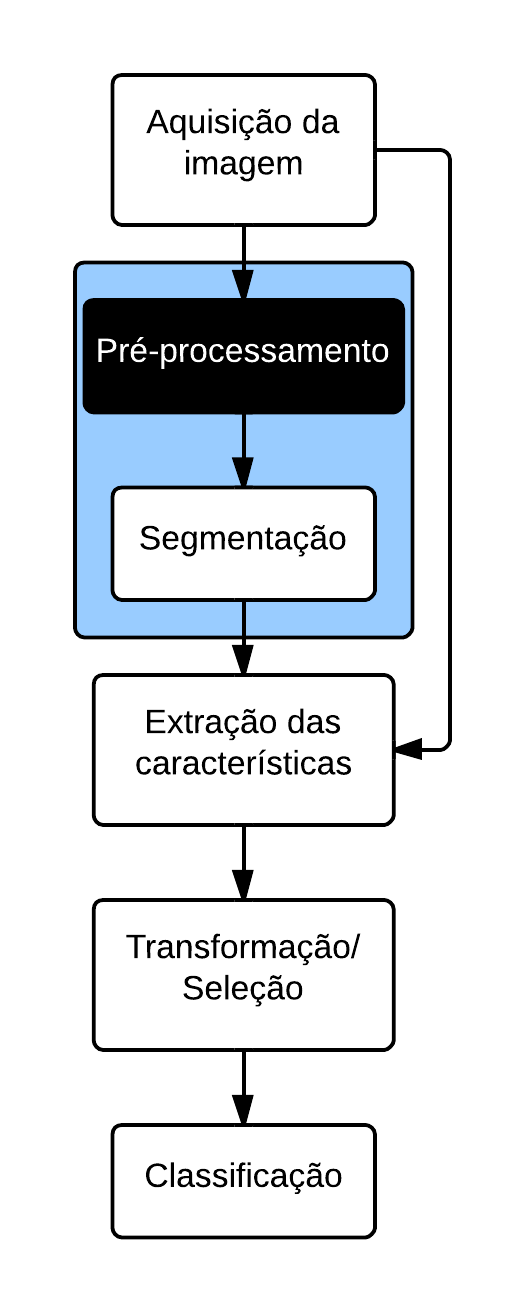
\includegraphics[width=0.3\linewidth]{figuras/flow.png}
 \end{center}
 \caption[Etapas canônicas do reconhecimento de padrões desde a aquisição da imagem até sua posterior classificação.]{Etapas canônicas do reconhecimento de padrões desde a aquisição da imagem até sua posterior classificação. As etapas de pré-processamento e segmentação --- apresentadas em destaque --- são normalmente pouco exploradas, quando comparadas com as etapas posteriores. O enfoque desse estudo é dar maior atenção à etapa de pré-processamento. \textit{Fonte:~Elaborado pela autora.}}
 \label{fig:fluxo}
\end{figure}

\enlargethispage{-\baselineskip}

O desbalanceamento de classes também se apresenta como um obstáculo para que a classificação de imagens seja satisfatória. Esse problema é caracterizado pela diferença entre o número de exemplos disponíveis para cada classe da base de imagens. Muitos métodos de transformação do espaço de características e de classificação assumem que as classes da base estão balanceadas, o que nem sempre é verdade. Portanto, é proposto a geração de imagens artificiais a partir do processamento das imagens originais, com o objetivo de rebalancear a base de imagens e consequentemente o modelo criado para a classificação. De maneira sumária, {\textbf esta pesquisa busca melhorar a classificação de imagens, utilizando métodos de processamento com foco na extração de características latentes e no rebalanceamento de classes.} Esse método foi comparado com o SMOTE, técnica de sobreamostragem dos vetores de características ao interpolar os exemplos mais próximos.

Os resultados obtidos, posteriormente apresentados na Seção \ref{sec:resultados}, demonstram o potencial da geração de imagens artificiais. A visualização do espaço de características após o rebalanceamento das classes é crucial para analisar se as novas características extraídas são relevantes, ou seja, se adicionaram informações que estavam latentes ao aprendizado. De maneira sumária, {\textbf esta pesquisa busca melhorar a classificação de imagens, utilizando métodos de processamento com foco na extração de características latentes e no rebalanceamento de classes.}

%--------------------------------------------------------------------------------
\section{Contextualização}

O grupo de pesquisa em Visualização, Imagens e Computação Gráfica (VICG), do Instituto de Ciências Matemáticas e de Computação (ICMC), tem atuado nas áreas de apoio para a classificação de coleções de imagens. Os trabalhos do grupo estão relacionados à visualização de informação com projeções multidimensionais e árvores~\cite{Joia2011}, assim como à extração de características e classificação de coleções de imagens~\cite{Paiva2011}. No que tange o processamento de imagens digitais, \citeonline{Picon2011} e \citeonline{Ponti2013} focaram no pré-processamento para obter melhores resultados de classificação.

\citeonline{Paiva2011} mostraram que os espaços de características formados por cor e textura podem ser melhorados, porém há um limite até o qual as características podem ser transformadas, ou selecionadas, de forma a garantir a discriminação entre as classes. Tal projeto atua na investigação de métodos que permitam gerar espaços de características com maior discriminação entre as classes, facilitando a classificação.

Em outros dois trabalhos relacionados é possível ver a diferença na performance para problemas de classificação de imagens. No primeiro, os autores atingem acurácia acima de 98\% na classificação de frutas após investigar alterações nos parâmetros de aquisição, realizar pré-processamento e obter a segmentação \cite{Rocha2010}. No segundo, os autores indicam que o método utilizado para obter a imagem em escala de cinza (comumente utilizada por algoritmos de extração), pode impactar significativamente a classificação final de diversas bases de imagens~\cite{Kanan2012}.

Recentemente, \citeonline{Ponti2014} demonstraram que o uso de algoritmos de pré\hyp{}processamento permite ao mesmo tempo obter vetores de características mais compactos e com maior capacidade de discriminação entre classes.


% \meutodo{Na literatura \citeonline{Peng2014} exploraram a geração de imagens artificiais a partir de modelos 3D CAD}

%--------------------------------------------------------------------------------
\section{Relevância e hipóteses}

Conforme anteriormente mencionado, muitos aspectos influenciam a performance da classificação de coleções de imagens. É comum encontrar bases cuja extração de características é considerada difícil, onde algoritmos canônicos de extração não conseguem extrair características que diferenciem bem as classes, prejudicando sua posterior classificação. Normalmente, tenta-se lidar com as particularidades das características extraídas através de transformações no espaço de atributos ou mesmo projetando classificadores mais elaborados. Acredita-se que, ao invés disso, é importante investigar métodos de processamento e preparação de imagens antes da extração das características. Por isso, {\textbf uma das hipóteses desse trabalho é que o uso desses métodos possa revelar características latentes -- não visíveis nas imagens originais -- que podem melhorar a acurácia da classificação.}


Além disso,
% uma ampla variedade de classificadores e de transformações assume que as classes da base estão balanceadas.
o desbalanceamento de classes é um obstáculo para uma classificação satisfatória, e por isso também será estudado.
% Outro fator de impacto em tal acurácia é o desbalanceamento de classes nas bases de dados para pesquisa.
Em bases médicas, por exemplo, a quantidade de imagens relacionadas com uma doença rara é menor do que as imagens de pacientes sem a doença. Nessas situações, em que as imagens representam eventos importantes porém menos frequentes, o sistema de classificação pode ter problemas para lidar com a classe minoritária. {\textbf A hipótese, nesse caso, é que a geração de imagens artificiais como preparação para a extração de características pode melhorar a acurácia da classificação, quando comparada à geração de exemplos artificiais no espaço de atributos.} Ou seja, gerar novas imagens artificiais — que serão posteriormente reduzidas a atributos — pode apresentar melhores resultados para a classificação do que o \textit{bootstrap} de atributos artificiais.

\meutodo{hipóteses repetidas?}

\begin{itemize}
\item A geração de imagens artificiais pode contribuir com o balanceamento entre classes (em se tratando de problemas de classes desbalanceadas), melhorando a acurácia de algoritmos de classificação, quando comparada à geração de exemplos artificiais no espaço de atributos;
\item O uso de métodos de pré-processamento permite a extração de características latentes que aumentem a variância entre as classes, sem aumentar, no entanto, a variância intra-classe. Melhorando, assim, a classificação.
\end{itemize}

%--------------------------------------------------------------------------------
\section{Contribuições}

O objetivo desta pesquisa é explorar as etapas de processamento de imagens com o intuito de melhorar a discriminação entre classes de uma coleção de imagens.

Após gerar as imagens artificiais, somente as imagens relevantes serão incluidas no treinamento. Por fim, conforme descrito na Seção \ref{sec:resultadospreliminares} de resultados preliminares, será possível analisar operações simples e canônicas de pré-processamento de imagens.

Dados tais aspectos, pode-se então diferenciar os objetivos gerais e específicos:

\begin{description}
\item[Geral] \

Investigar os métodos de pré-processamento de imagens de forma a preparar uma coleção de imagens para a extração de características. Com isso, espera-se ao mesmo tempo obter características latentes e balancear o número de instâncias de diferentes classes.

\item[Específicos] \

  \begin{itemize}
      \item Analisar o impacto da utilização de métodos canônicos de pré-processamento, como filtragem, adição de ruído e mistura, na classificação de bases de imagens.

      % obter alterações na imagem que permitam extrair as características latentes, que não são visíveis nem diretamente passíveis de extração, na imagem original;

      \item Modificar a base de imagens original de forma a tornar as características latentes visíveis. Com isso, pretende-se aumentar a variância entre as classes -- antes da extração de características e classificação -- com o auxílio dos métodos canônicos e CNN;

      \item Gerar imagens artificiais a partir das imagens pertencentes às classes minoritárias, compensando o desbalanceamento.
  \end{itemize}
\end{description}

Considerando os objetivos aqui descritos, os resultados esperados desta pesquisa estão destacados na Seção \ref{sec:resultados}.

%--------------------------------------------------------------------------------
\section{Estrutura do documento}

O conteúdo desta dissertação está estruturado como segue.

\begin{description}
\item [Capítulo~\ref{cap:revisao}:] são conceituados os principais fundamentos necessários para o desenvolvimento desta pesquisa: pré-processamento de imagens, extração de características e desbalanceamento de classes.

\item [Capítulo~\ref{cap:quantization}:] a redução do número de intensidades de cor antes da extração de características é descrita.

\item [Capítulo~\ref{cap:metodo}:] descreve-se os métodos para a geração artificial de imagens com o objetivo de rebalancear classes.

\item [Capítulo~\ref{cap:resultados}:] apresenta e discute os resultados.
% a proposta é retomada ao indicar como será resolvido o problema do desbalanceamento e a melhoria das imagens com base nas suas características latentes.

\item [Capítulo~\ref{cap:conclusoes}:]

\end{description}
